\documentclass[10pt, t]{beamer}
% \usepackage[UTF8]{ctex}
\usepackage{amsmath}
\usepackage{setspace}
\usepackage{float}
\usepackage{multido}
\usepackage{multirow}
\usepackage{array}
\usepackage{enumerate}
\usepackage{booktabs}
\usepackage{indentfirst}
\usepackage[style=mla]{biblatex}
\usepackage{setspace}
\usepackage{subcaption}
\usepackage{hyperref}
\usepackage{textpos}
% \usepackage{fontspec}

% \beamerdefaultoverlayspecification{<+->}
\makeatletter
\let\@@magyar@captionfix\relax
\makeatother

\definecolor{bladerunnerblue}{RGB}{41, 159, 163}
\definecolor{bladerunnerred}{RGB}{194,84,97}
\definecolor{themecolor}{RGB}{25,25,112}
\definecolor{weak}{RGB}{150,150,150}

\renewcommand{\emph}[1]{{\color{themecolor}\textsl{#1}}}
\newcommand{\alarm}[1]{{\color{bladerunnerred}{#1}}}
\newcommand{\N}{\mathbb{N}}
\newcommand{\R}{\mathbb{R}}
\newcommand{\dom}{\operatorname{dom}}
\newcommand{\myseries}[2]{$#1_1,#1_2,\dots,#1_#2$}
\newcommand{\nullspace}{~\\[15pt]}
\newcommand{\remark}{\textbf{Remark: }}
\newcommand{\question}{\textbf{Question: }}
\newcommand{\scp}[2]{\langle\,#1\,,\,#2\,\rangle} \newcommand{\scpp}{\langle\,\cdot\,,\,\cdot\,\rangle}
\newcommand{\weaken}[1]{{\color{weak}\textit{#1}}}
\newcommand{\underover}[3]{\underset{#2}{\overset{#3}{#1}}}
\renewcommand{\emptyset}{\varnothing}


\usetheme{Madrid}
\setbeamertemplate{navigation symbols}{}

\addtobeamertemplate{frametitle}{}{
\begin{textblock*}{100mm}(0.85\textwidth,-1cm)
\includegraphics[height=1cm]{../../logo.png}
\end{textblock*}}


\usecolortheme[named=themecolor]{structure}

\setbeamertemplate{items}[default]

\hypersetup{
    colorlinks=true,
    linkcolor=themecolor,
    filecolor=themecolor,
    urlcolor=themecolor,
    citecolor=themecolor,
}

\title{VV186: Honors Mathematics}
\subtitle{Integral}
\institute[UM-SJTU JI]{Univerity of Michigan-Shanghai Jiao Tong University Joint Institute}
\author{Xingjian Zhang}

\begin{document}

\begin{frame}
    \titlepage
    \begin{center}
        \includegraphics[height=2cm]{../../logo2.png}
    \end{center}
\end{frame}

\begin{frame}
    \frametitle{Outline}
    \begin{spacing}{1}
        \tableofcontents
    \end{spacing}
\end{frame}

\section{Notions of Integration}
\subsection{Hierarchy of Integrals}
\begin{frame}
    \frametitle{Hierarchy of Integrals}
    \begin{enumerate}
        \item Integral of step functions
        \item Regulated integral
        \item Darboux integral \& Riemann Integral
        \item Lebesgue integral
        \item Gauge integral (Henstock-Kurzweil integral)
    \end{enumerate}
    \textbf{Remark:} We only study the first three hierarchies. Make sure you remember their definitions and properties.
\end{frame}

\subsection{Step Functions}
\begin{frame}
    \frametitle{Step Functions}
    \begin{figure}[H]
        \centering
        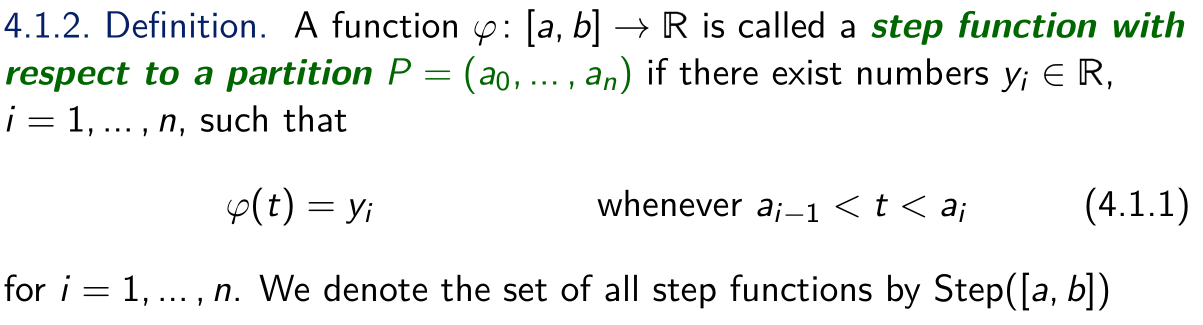
\includegraphics[width=0.9\textwidth]{2020-12-05-11-51-42.png}
    \end{figure}
    \textbf{Remark:} We can arbitrarily define $\varphi$ at points $a_i$ and $\varphi$ is still a step function. For example, 
    \begin{figure}[H]
        \centering
        
\includegraphics[width=0.9\textwidth]{2020-12-05-11-54-33.png}
    \end{figure}
    \textbf{Remark:} $\operatorname{Step}([a,b])$ is a vector space. $\int$ is linear, and does not depend on values on finite sets (To be more precise, on 0-measure set).
\end{frame}

\subsection{Regulated Integral}
\begin{frame}
    \frametitle{Regulated Functions}

    \begin{figure}[H]
        \centering
        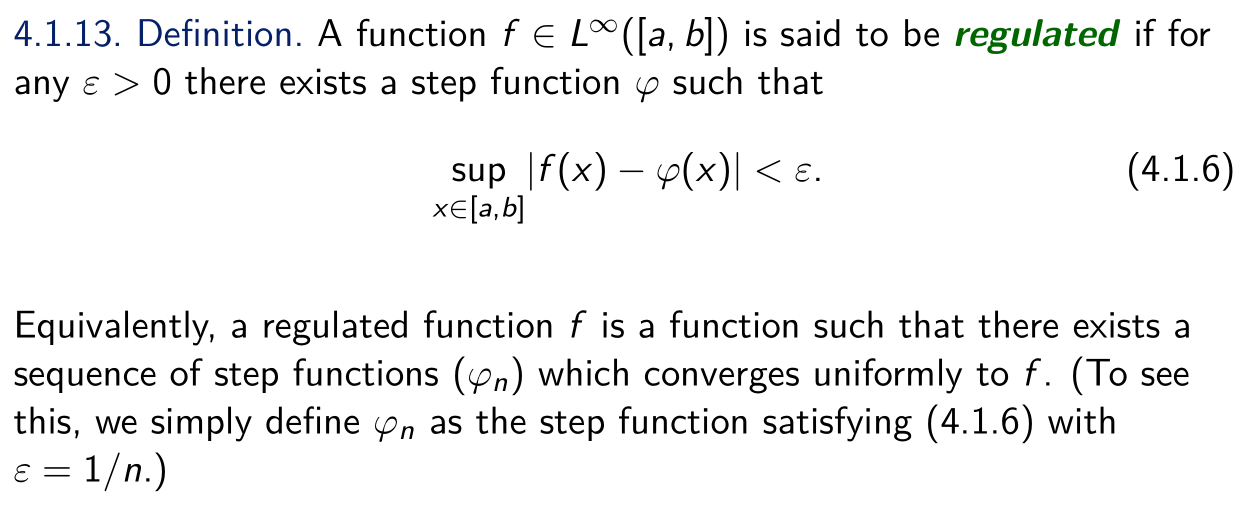
\includegraphics[width=0.9\textwidth]{2020-12-02-11-57-35.png}
    \end{figure}

    \textbf{Remark:}
    \begin{itemize}
        \item The \textit{equivalent description} of 4.1.13. Definition is more intuitive: We seek for a sequence of step functions that converge \textbf{uniformly} to the target function.
        \item The continous a.e.\footnote[frame]{``a.e.'' is the abbreviate of ``almost everywhere''.} functions on a closed interval are regulated. i.e. $\mathrm{PC}([a,b])\subset\mathrm{Reg}([a,b])$
    \end{itemize}

\end{frame}

\begin{frame}
    \frametitle{Regulated Integral}
    \begin{figure}[H]
        \centering
        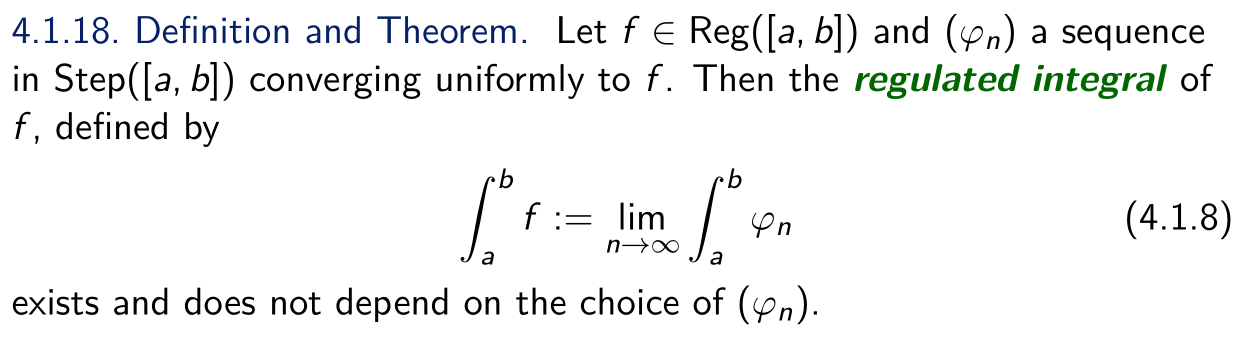
\includegraphics[width=0.9\textwidth]{2020-12-02-12-08-32.png}
    \end{figure}
    \begin{figure}[H]
        \centering
        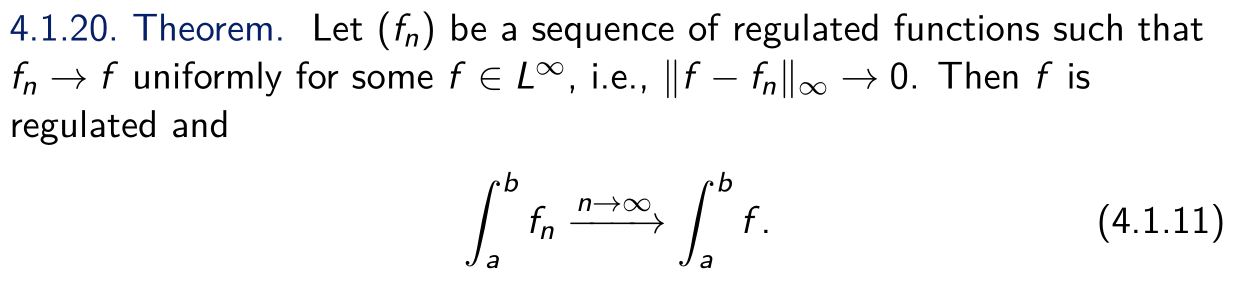
\includegraphics[width=0.9\textwidth]{2020-12-02-12-09-22.png}
    \end{figure}
\end{frame}

\begin{frame}
    \frametitle{Exercise}
    Consider the function
    \begin{figure}[H]
        \centering
        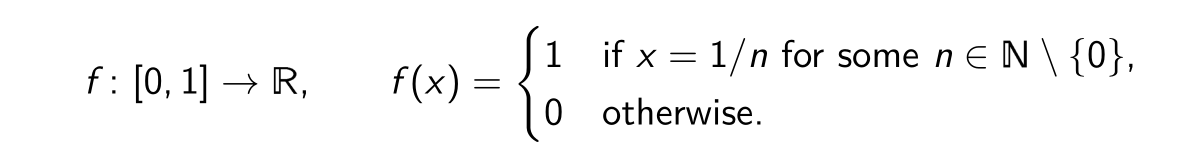
\includegraphics[width=0.9\textwidth]{2020-12-02-12-24-56.png}
    \end{figure}
    Is the function regulated?
\end{frame}

\begin{frame}
    \frametitle{Exercise}
    True or False?
    \begin{enumerate}
        \item $f(x)=x^3+e^x$ on $[-1,1]$ is regulated.
        \item
              Since $f(x)=x^{2}$ is regulated on each $[-n, n],$ where $n \in \mathbb{N}, f$ is regulated on $\mathbb{R}$
              because we can let $n \rightarrow \infty$
        \item A continuous function is piecewise continuous
        \item Let $f,$ g be two real-valued function defined on $[0,1] .$ Furthermore, assume $f-g=x,$ then the equation $\int_{0}^{1}(f-g)=\int_{0}^{1} f-\int_{0}^{1} g=\frac{1}{2}$ holds.
        \item Let $f \in \operatorname{Reg}([0,1]),$ let $g$ be a real-valued function. Then $f \circ g$ is regulated.
    \end{enumerate}
\end{frame}

\subsection{Darboux Integral}
\begin{frame}
    \frametitle{Darboux Integral}
    \begin{figure}[H]
        \centering
        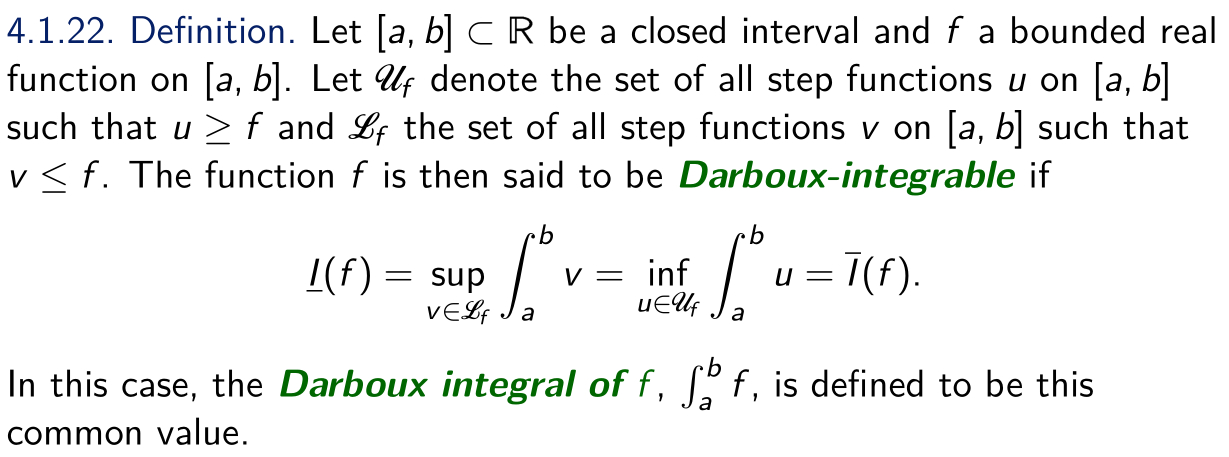
\includegraphics[width=0.9\textwidth]{2020-12-02-12-11-33.png}
    \end{figure}
    \textbf{Question: }True or false?\\
    If $\int_a^b|f|$ is Darboux integrable, $\int_a^b f$ is Darboux integrable.
\end{frame}

\begin{frame}
    \frametitle{Exercise}
    Consider the function
    \begin{figure}[H]
        \centering
        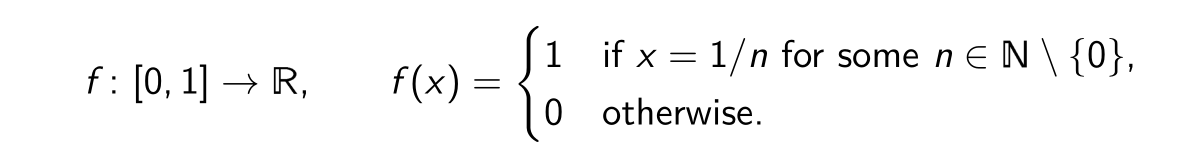
\includegraphics[width=0.9\textwidth]{2020-12-02-12-24-56.png}
    \end{figure}
    Is the function Darboux integrable?
    \nullspace\pause
    \textit{General Strategy}\\
    \begin{itemize}
        \item construct a sequence of step functions $(u_n)>f$,
        \item construct a sequence of step functions $(l_n)<f$,
        \item find $\int u_n$ and $\int l_n$,
        \item verify $\underset{n\to \infty}{\lim}\int u_n = \underset{n\to \infty}{\lim}\int l_n$.
    \end{itemize}

\end{frame}

\subsection{Riemann Integral}
\begin{frame}
    \frametitle{Riemann Integral}
    \begin{figure}[H]
        \centering
        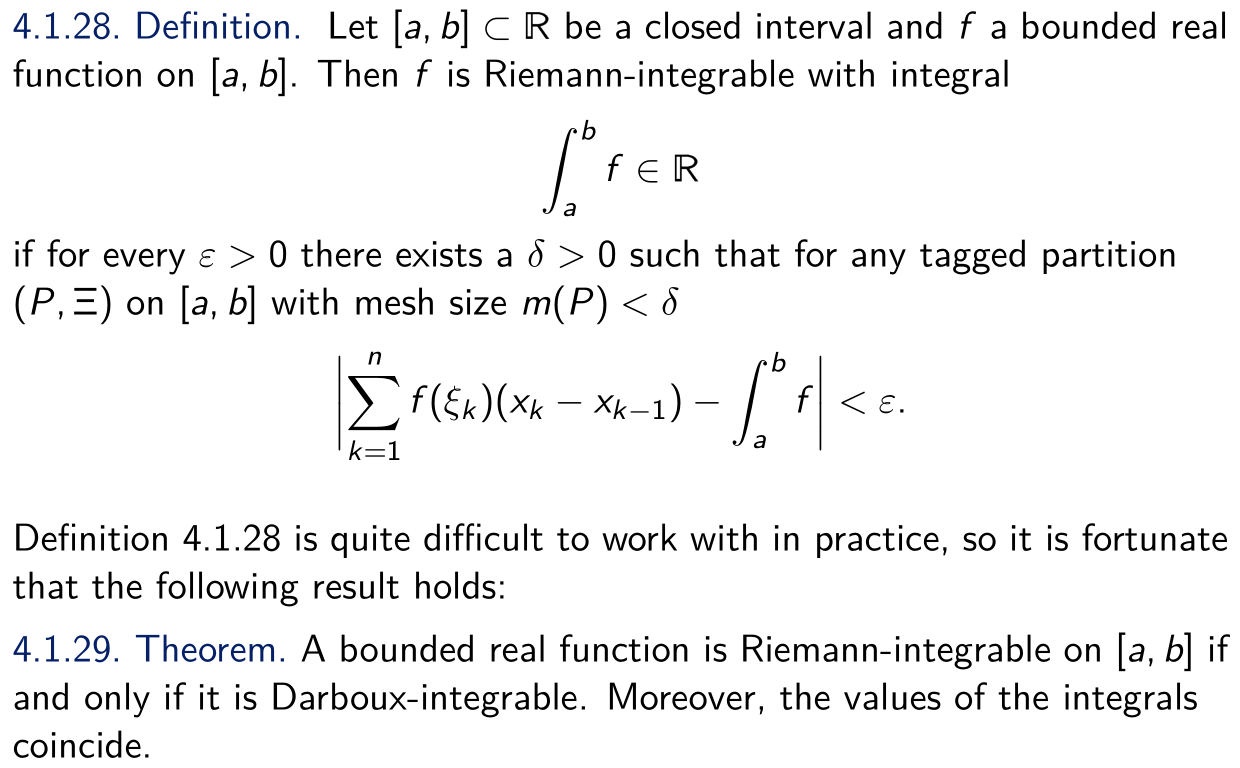
\includegraphics[width=0.9\textwidth]{2020-12-02-12-12-35.png}
    \end{figure}
\end{frame}

\begin{frame}
    \frametitle{Darboux Integral vs. Riemann Integral}
    Describe in words the difference between \textbf{Darboux Integral} and \textbf{Riemann Integral}. How are these two concepts different? If you can, state some properties that they have in common or that serve to differentiate them from each other. Is one of them also always an example of the other? Give examples.
    \nullspace
    This exercise is left for you!
\end{frame}

\begin{frame}
    \frametitle{Mean Value Theorem of Integral Calculus}

    \textit{From Assignment}\nullspace

    Let $[a,b]\subset\R$ be a closed interval and $f:[a,b]\to\R$ a continuous real function. Then there exists a $\xi \in (a,b)$ such that
    $$\int_a^bf(x)dx=(b-a)f(\xi).$$

\end{frame}

\begin{frame}
    \frametitle{Not End}
    \vspace{1cm}
    \begin{center}
        \LARGE
        Forever\\
        Have Fun \\
        And \\
        Learn Well!\footnote[frame]{Special acknowledgement to former TA \textbf{Zhang Leyang}, who offered plenty of exercises and advice to my recitation class.}
    \end{center}
\end{frame}

\end{document}